\documentclass[12pt, a4paper]{article}

% Ru lang stuff
\usepackage [utf8x] {inputenc}
\usepackage [T2A] {fontenc}

% running titles 
\usepackage{fancybox}
\usepackage{fancyhdr}

% for last page number
\usepackage{lastpage}

%for colored tablets cells
\usepackage{colortbl}

% for Ru text in formulas
\usepackage[warn]{mathtext}

% for captions 
\usepackage[labelsep=period]{caption}
\usepackage{capt-of}

% for colored hyperrefs
\usepackage{xcolor}
\usepackage{hyperref}

% for pictures 
\usepackage{graphicx}

% for coll math
\usepackage{amsmath}

% path to all pictures
\graphicspath{{picks/}}

% for enumerates
\usepackage[shortlabels]{enumitem}

% for diff running titles on pages with diff parity
\usepackage{ifthen}
\usepackage{pdfpages}
\usepackage[strict]{changepage}

%for drawings
\usepackage{tikz}
\usetikzlibrary{calc}
\usetikzlibrary{decorations.pathmorphing}

% for good text in tablets
\usepackage{array}

% upgrading tables
\newcolumntype{P}[1]{>{\centering\arraybackslash}p{#1}}
\newcolumntype{M}[1]{>{\centering\arraybackslash}m{#1}}


% dock fields 20 15 15 35
\usepackage[left=12mm, top=12mm, right=15mm, bottom=28mm, nohead, footskip=10mm]{geometry}

% for cool tables
\usepackage{multirow}

% for different section/subsection/subsubsection styles in contents and doc
\usepackage[english, russian]{babel}

\usepackage{amsmath}

% for cool tables
\usepackage{tabularx}

\newcommand{\sect}[2] {
    \addtocounter{section}{1}
    \section*{\Huge\thesection.\,#1}
    \addcontentsline{toc}{subsection}{ \texorpdfstring{\thesection.\qquad\qquad #2}{Lg}}
}

\newcommand{\subsec}[2] {
    \addtocounter{subsection}{1}
    \subsection*{\thesubsection.\,#1}
    \addcontentsline{toc}{subsection}{ \texorpdfstring{\quad \thesubsection.\qquad\ #2}{Lg}}
}

\newcommand{\subsubsec}[2] {
    \addtocounter{subsubsection}{1}
    \subsubsection*{\thesubsubsection.\,#1}
    \addcontentsline{toc}{subsection}{ \texorpdfstring{\quad\quad\ \thesubsubsection. #2}{Lg}}
}
%-------------------------------------------------------------------------%

% for easy mini pages with shifts
\newcommand{\shiftedText}[3]{
\hspace*{#1}\begin{minipage}[t]{#2}
#3
\end{minipage}
}

\newcolumntype{P}[1]{>{\centering\arraybackslash}p{#1}}

% page style setup (for running titles)
\fancypagestyle{plain}{ %
\fancyhf{} % remove everything

 % lines parameters
\renewcommand{\headrulewidth}{0pt}
\renewcommand{\footrulewidth}{0pt}

% running titles contents
\fancyfoot[L]{\ifthenelse{\isodd{\thepage}}{Работа 1.4.1}{\thepage}}
\fancyfoot[R]{\ifthenelse{\isodd{\thepage}}{\thepage}{Работа 1.4.1}}
}

% choosing page style with our running titles
\pagestyle{plain}

\tolerance = 10000

\title{Лабораторная работа №1.4.1}
\author{Mikhail Pavlov \thanks{MIPT}}
\date{October, 2021}
\begin{document}


\shiftedText{0.5cm}{14cm}
{
    \begin{center}
    \vspace*{1.0cm}    
        
        {\bf\Huge Работа 1.4.1 }
        
    \vspace*{0.2cm}    
        
        {\bf\LARGE Изучение экспериментальных погрешностей на примере физического маятника }
        
    \vspace*{0.8cm}
        {\LARGE Работу выполнил Павлов Михаил Б01-109 }
        
    \vspace*{1.6cm}
    
    \end{center}
}

\fancypagestyle{plain}{ %
\fancyhf{} % remove everything

 % lines parameters
\renewcommand{\headrulewidth}{0pt}
\renewcommand{\footrulewidth}{0pt}
% running titles contents
\fancyfoot[L]{\ifthenelse{\isodd{\thepage}}{Работа 1.4.1}{\thepage}}
\fancyfoot[R]{\ifthenelse{\isodd{\thepage}}{\thepage}{Работа 1.4.1}}
}

% choosing page style with our running titles
\pagestyle{plain}

\tolerance = 10000

\vspace*{0.6cm}

        {\Large 1. Аннотация \\}
        \noindent\begin{minipage}[c]{0.67\textwidth}
            \hspace{1cm}
            Физическим маятником называют твёрдое тело, способное совершать колебания в вертикальной плоскости,
            будучи подвешено за одну из своих точек в поле тяжести.
            Основное отличие физического маятника от математического в том, что маятник не является точечным объектом,
            а представляет собой совокупность жёстко связанных точечных масс. В данной работе в качестве такого маятника
            используется тонкий однородный металлический стержень, подвешиваемый в некоторой точке с помощью небольшой опорной призмы (см. рис. 1). Острое ребро
            призмы, опирающееся на подставку, задаёт ось качания
            (или вращения) маятника.
        \end{minipage}
        \begin{minipage}[c]{0.32\textwidth}
            \begin{center}
                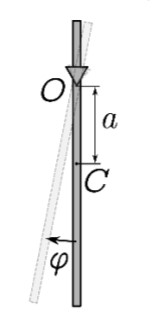
\includegraphics[scale=0.6]{Pics/picture1.jpg} \\
                \textit{\textcolor[HTML]{000000}{Рис. 1. Стержень \\ как физический маятник}}
            \end{center}
        \end{minipage}  
        Закон, описывающий вращательное движение твёрдого тела вокруг
        фиксированной оси, аналогичен второму закону Ньютона. Получим его для
        простейшего случая точечной массы.
        Как известно, для динамики движения точечной массы 𝑚𝑚 под действием
        силы 𝐹𝐹 вдоль некоторой прямой справедливо уравнение Ньютона
        \begin{displaymath}
            F = \frac{dp}{dt}
        \end{displaymath}
        где $p = mv$ --- импульс, $v$ - скорость тела. \\
        

        {\Large 2. Теоретические сведения \\}
        Величину $J = mr^2$ называют \textit{моментом инерции} точечного тела.
        В законе вращательного движения момент инерции играет роль,
        аналогичную массе тела при поступательном движении.

        В случае твердого тела, состоящего из совокупности материальных точек, вращающихся вокруг
        фиксированной оси под моментом инерции следует понимать сумму (интеграл) по всем точкам тела:
        \begin{displaymath}
            J = \sum_{i}^{} m_ir_i^2  
        \end{displaymath}
        где $r_i$ --- расстояние от точки массой $m_i$ до оси вращения. Видно, что момент инерции зависит от массы тела, его формы, а также от положения оси
        вращения. Момент инерции тонкого стержня массой $𝑚$ и длиной $𝑙$, вращающегося вокруг оси,
        проходящей через центр масс, равен
        \begin{displaymath}
            J_C = \frac{ml^2}{12}
        \end{displaymath}
        А момент инерции стержня, подвешенного на расстоянии 𝑎𝑎 от центра масс,
        может быть вычислен по теореме Гюйгенса–Штейнера:
        \begin{equation}
            J = \frac{ml^2}{12} + my^2.
        \end{equation}
        В частности, если стержень подвесить за один из концов, то $y = l/2$ и $J = ml^2/3$.

        Чтобы получить формулу периода колебаний физического маятника,
        воспользуемся аналогией с пружинным маятником, период колебаний которого равен, как известно, $𝑇 = 2\pi\sqrt{𝑚/𝑘}$. Здесь роль массы 𝑚, как мы уже
        обсудили, играет момент инерции тела 𝐽, а роль коэффициента жёсткости
        пружины 𝑘 — коэффициент пропорциональности между моментом силы и
        величиной отклонения 𝑚gy. Таким образом, приходим к следующей общей формуле для периода колебаний произвольного физического маятника:
        \begin{equation}
            T = 2\pi\sqrt{\frac{J}{mgy}}
        \end{equation}
        А для стержня длиной 𝑙, подвешенного на расстоянии 𝑎 от центра, получаем:
        \begin{equation}
            T = 2\pi\sqrt{
                \frac{
                    \frac{l^2}{12} + y^2}
                    {gy}
            }
        \end{equation}

        {\Large 3. Экспериментальная установка \\}
        Если на стержень насадить груз, то момент инерции маятника, а значит
        и период его колебаний, будет зависеть от положения груза относительно
        оси качания. Момент инерции маятника будет равен
        \begin{displaymath}
            J = J_0 + m_ry^2
        \end{displaymath}
        \noindent\begin{minipage}[c]{0.67\textwidth}
            \hspace{1cm}
            Заметим, что величину $𝑦$ на практике измерить напрямую затруднительно, поскольку положение центра масс
            груза точно не известно. Вместо этого можно измерить
            положение центра масс маятника с грузом и без него.
            Пусть $𝑥_{c0}$ --- расстояние от точки подвеса (острия
            призмы) до центра масс маятника без груза. Тогда центр
            масс маятника с грузом находится в точке
            \begin{displaymath}
                x_c = \frac{m_0x_{c0} + m_ry}{M}
            \end{displaymath}
            где $𝑚_0$ — масса маятника без груза (стержня вместе с
            призмой), $𝑀 = 𝑚_0 + 𝑚_r$ — полная масса маятника. Положения центра масс $x_c$ и $𝑥_{c0}$ могут быть измерены с
            помощью подставки. Отсюда находим формулу для вычисления положения центра масс груза:
        \end{minipage}
        \begin{minipage}[c]{0.32\textwidth}
            \begin{center}
                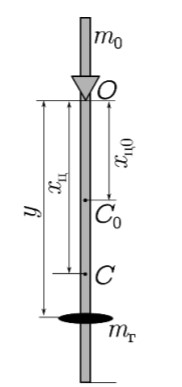
\includegraphics[scale=0.6]{Pics/picture2.jpg} \\
                \textit{\textcolor[HTML]{000000}{Рис. 2. Маятник с \\ дополнительным грузом}}
            \end{center}
        \end{minipage}
        \begin{equation}
            y = \frac{Mx_c - m_0x_{c0}}{m_r}
        \end{equation}

        Из общей формулы найдём период колебаний маятника грузом:
        \begin{equation}
            T = 2\pi{\frac{J_0 + m_ry^2}{gMx_c}}.
        \end{equation}

        {\Large 4. Инструментальные погрешности \\}
        \textbf{Линейка: } $\sigma_{rul} = \pm 0.5$ мм. (половина цены деления)\\
        \textbf{Электронные весы: } $\sigma_{v} = \pm 0.1$ r (маркировка производителя) \\
        \textbf{Счетчик колебаний: } $\sigma_{cnt} = \pm 0.01c$ (маркировка производителя) \\
        \newpage
        Пробный эксперимент:
        \begin{center}
            \begin{tabular}{ | c | c | c | c | }
                \hline
                N & n & $\tau$, c & T, c \\ \hline
                1 & 20 & 30.56 & 1.53 \\ \hline
                2 & 20 & 30.56 & 1.53 \\ \hline
                3 & 20 & 30.56 & 1.53 \\ \hline
                4 & 20 & 30.56 & 1.53 \\ \hline
            \end{tabular}
            \end{center} 
        Случайная погрешность равна 0, так что общая погрешность счетчика колебаний равна систематический погрешности.
            
        \vspace*{0.3cm}
        {\Large 5. Результаты измерений и обработка данных \\} 
        {\textbf{Измерение масс:}}
        $m_0 = 1637,6r$ - масса штанги \\
        $m_r = 348,7r$ - масса груза \\
        Поскольку погрешность измерения массы груза несоизмерима мала по сравнению с этими значениями, то относительную погрешность можно считать равной 0. \\
        {\textbf{Измерение длинн:}}
        $x_{np} = 239$мм - расстояние от ближайшего края штанг до призмы \\
        $x_{c0} = 261$мм - расстояние от призмы до центра масс штанги \\
        $l = 1000$мм - длина штанги \\
        $\epsilon = 0.18\%$ - относительная погрешность измерения расстояния до центра масс.
        
        \begin{center}
            \begin{tabular}{ | c | c | c | c | c | c | c | c | }
                \hline
                N & y, мм & n & $\tau$, c & T, с & g, м/$c^2$ & $x_c$, мм & $\Delta y,$ мм \\ \hline
                1 & 580,00 & 25 & 38,6	& 1,54 & 9,041 & 317 & 0 \\ \hline
                2 & 528,72 & 25 & 38,2	& 1,53	& 9,187 & 308	& 40 \\ \hline
                3 & 483,16 & 25 & 37,6	& 1,51 	& 9,400 & 300	& 80 \\ \hline
                4 & 437,59 & 25 & 37,3  & 1,49	& 9,526 & 292	& 120 \\ \hline
                5 & 397,71 & 25 & 37,0  & 1,48	& 9,632 & 285	& 160 \\ \hline
                6 & 363,53 & 25 & 36,7	& 1,47  & 9,722 & 279 	& 200 \\ \hline
                7 & 323,66 & 25 & 36,5	& 1,46	& 9,776 & 272	& 240 \\ \hline
                8 & 283,79 & 25 & 36,4	& 1,46	& 9,804 & 265	& 280 \\ \hline
                9 & 249,61 & 25 & 36,3	& 1,45	& 9,807 & 259	& 320 \\ \hline
                10 & 186,95 & 25 & 36,4	& 1,45	& 9711  & 248	& 380 \\ \hline
            \end{tabular}
            \captionof{table}{Результаты расчета g.}
            \end{center} 
    
            Получаем, что $\overline{g} = 9,56$ м/$с^2$ \\
            Относительная погрешность $\epsilon \approx 2,5\%$ 
            
            \begin{minipage}[c]{\textwidth}
                \begin{center}
                    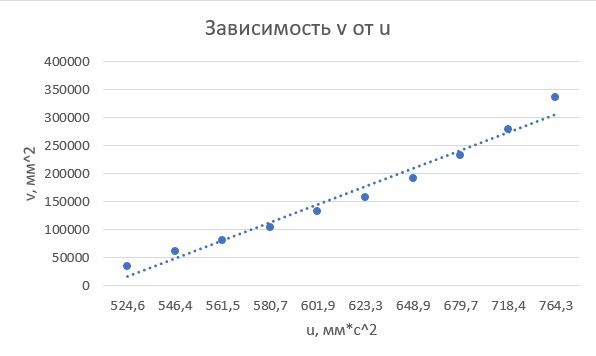
\includegraphics[scale=1]{Pics/picture3.jpg} \\
                    \textit{\textcolor[HTML]{000000}{Рис. 3. График зависимости v от u}}
                \end{center}
            \end{minipage}

            Здесь $v = y^2, a u = T^2x_c.$
            По рисунку отчетливо видно, что экспериментальные точки графика хорошо ложатся на прямую линию в пределах погрешности.

            Теперь перейдем к графику зависимости периода колебаний от расстояния от центра масс до груза.

            \begin{minipage}[c]{\textwidth}
                \begin{center}
                    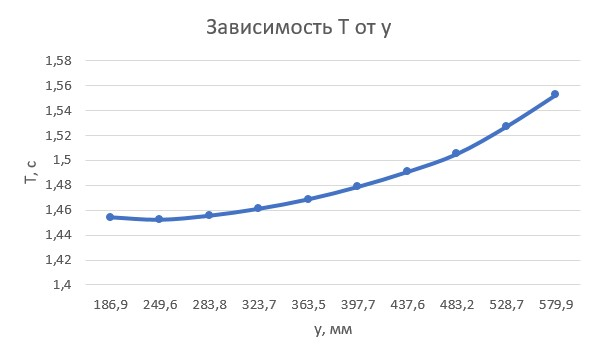
\includegraphics[scale=1]{Pics/picture4.jpg} \\
                    \textit{\textcolor[HTML]{000000}{Рис. 4. График зависимости T от y}}
                \end{center}
            \end{minipage}
            \vspace*{0.3cm}
            
            Как видим, наш график имеет минимум в точке 2. То есть период колебания физического маятника в этой точке минимальный.
            Это вполне логично, если учитывать, что T по формуле (3) зависит от y. 
            Как раз в точке минимума у нас $y$ минимальный
            \vspace*{0.3cm}

    
            {\Large 5. Вывод: \\}

            Стоит отметить, что в ходе данной лабораторной работы нам не удалось получить значение g
            в пределах погрешности. Однако, все это вполне объяснимо, так что неудачным эксперимент
            тоже назвать нельзя. Значения g получились не самыми точными, из-за того что мы считали 
            призму невесомой, хотя по факту она влияла на положение центра масс и на момент инерции.
            Но если внимательно изучить таблицу, то можно заметить, что в точках 8 и 9, где груз находился
            к центру масс ближе всего, значение g совпадает с табличным значением (9.81 м/$c^2$). И это не
            случайно, потому что чем ближе груз находится к центру масс, тем меньшее влияние он оказывает.
            Таким образом, можно быть вполне удовлетворённым результатом, полученным в опытах, где расстояние
            от центра масс до груза мало.    

\end{document}